\chapter{Análisis Teórico de la Aplicación del Internet de las Cosas en los Museos} \label{cap:analisis_teorico}

\addcontentsline{toc}{section}{Introducción}
        \textbf{\Large Introducción}\newline

        ...

    \section{Internet de las Cosas}

    El IoT como arquitectura emergente basada en la Internet global presta la posibilidad de intercambio de bienes y servicios entre redes de la cadena de suministro y que tiene un impacto importante en la seguridad y privacidad de los actores involucrados \cite{weber}. 
   
    \subsection{IoT en los museos internacionales}\label{sec:iotMundo}
        
        En el grupo de las bibliografías consultadas existen diversos ejemplos del empleo del IoT en los museos.

        En el caso del Conjunto Monumental de San Domenico Maggiore, ubicado en Nápoles (Italia), dentro del mismo se han transformado más de 270 esculturas en obras de arte parlantes. Equipado con un tablero de sensores, cada objeto puede proponerse automáticamente a los visitantes, compartiendo su historia en diferentes modalidades e idiomas, lo que permite un proceso de disfrute novedoso durante una experiencia cultural. \cite{monumentoSanDomenico}.
    
        En la Universidad de El Cairo, Egipto, desarrollaron un sistema para la conservación de las piezas en los museos, un sistema que no solo mide los atributos del entorno, sino que también mantiene la seguridad de los artefactos al detectar cualquier prueba de contacto o movimiento. También controla la intensidad de la luz en función de la ocupación de la sección del museo. Una característica diferenciadora del sistema es el diseño de energía ultrabaja de su nodo sensor que conduce a una larga vida útil de hasta 50 días. \cite{ultraLowPowerConservacion}.
    
        Estos son solo dos de los ejemplos. La tabla 1.2 muestra una relación de otros autores que emplean el IoT en los museos. Pero antes, para poder comprender la tabla 1.2 debemos definir una primera tabla en la que se le otorga a cada autor un número de manera tal que se entienda quien es cada autor. Por lo que se define la tabla 1.1:

    \begin{table}[H]
        \centering
        \caption{Numeración autores}
        \begin{tabular}{|c|c|}
        \hline
        \rowcolor[HTML]{9698ED} 
        Autor & Numeración Asociada \\ \hline
        Maksimovic y Cosovic \cite{maksimovic}     & 1                   \\ \hline
        Shah y Mishra \cite{shan}     & 2                                \\ \hline
        Marshall \cite{marshall}     & 3                                 \\ \hline
        Ghosh, Roy, y Saha \cite{ghosh}     & 4                          \\ \hline
        Rao, Sharma, y Narayan \cite{rao}     & 5                        \\ \hline
        Alletto y cols. \cite{alletto}     & 6                           \\ \hline
        Alsuhly y Khattab \cite{alsuhly}     & 7                         \\ \hline
        Spachos y Plataniotis \cite{spachos}     & 8                     \\ \hline
        (Lopez-Martínez, Iglesias, y Carrera \cite{lopezmartinez}     & 9\\ \hline
        \end{tabular}
        \label{tab:numeracion_autores}
    \end{table}

    \begin{table}[H]
        \centering
        \caption{IoT en los museos internacionales}
        \begin{tabular}{|l|l|l|}
        \hline
        \rowcolor[HTML]{9698ED} 
        Manifestación       & Mediciones                                                                                                                                                     & Tecnología                                                                                                                                              \\ \hline
        Temperatura         & {(}1,2,7{)} Temperatura °C                                                                                                                                     & \begin{tabular}[c]{@{}l@{}}{(}1{)} RPI, Sensores, Cloud\\ SVM (Árboles de Decisiones),\\ {(}2{)} IoT-WSMP,\\ {(}7{)} RPI, ESP32, Node-Red.\end{tabular} \\ \hline
        Humedad             & {(}1,2,7{)} Humedad \%                                                                                                                                         & \begin{tabular}[c]{@{}l@{}}{(}1{)} RPI, Sensores, Cloud\\ SVM (Árboles de Decisiones),\\ {(}2{)} IoT-WSMP,\\ {(}7{)} RPI, ESP32, Node-Red.\end{tabular} \\ \hline
        Intensidad luminosa & {(}2,7{)} Lumens                                                                                                                                               & \begin{tabular}[c]{@{}l@{}}{(}2{)} IoT-WSMP,\\ {(}7{)} RPI, ESP32, Sensores.\end{tabular}                                                               \\ \hline
        Vibraciones         & {(}1{)} Estabilidad del Edificio (Hz)                                                                                                                          & \begin{tabular}[c]{@{}l@{}}{(}1{)} RPI, Sensores, Cloud\\ SVM (Árboles de Decisiones).\end{tabular}                                                     \\ \hline
        Humo                & {(}1{)} C02 ppm                                                                                                                                                & \begin{tabular}[c]{@{}l@{}}{(}1{)} RPI, Sensores, Cloud\\ SVM (Árboles de Decisiones).\end{tabular}                                                     \\ \hline
        Polución            & {(}1{)} Polvo                                                                                                                                                  & \begin{tabular}[c]{@{}l@{}}{(}1{)} RPI, Sensores, Cloud\\ SVM (Árboles de Decisiones).\end{tabular}                                                     \\ \hline
        Xilófagos           & {(}1{)} Plagas de madera                                                                                                                                       & \begin{tabular}[c]{@{}l@{}}{(}1{)} RPI, Sensores, Cloud\\ SVM (Árboles de Decisiones).\end{tabular}                                                     \\ \hline
        Personas            & \begin{tabular}[c]{@{}l@{}}{(}7{)} Aceleracion, Toque.\\ {(}8{)} Geolocalización.\\ {(}3{)} Movimiento\\ {(}9{)} Propuestas de juegos en el museo\end{tabular} & \begin{tabular}[c]{@{}l@{}}{(}1{)} PIR, {(}4{)} IA,\\ {(}5{)} RPI, ESP32, Sensores.\end{tabular}                                                        \\ \hline
        \end{tabular}
        \label{tab:iot_internacional}
    \end{table}

    Como se puede observar en la tabla \ref{tab:iot_internacional} el mayor número de autores analizados centran su atención en el usuario que accede al museo en aras de brindarle una propuesta agradable en su visita.

    \section{Internet de las Cosas en Cuba}\label{sec:iotCuba} 

    En el contexto cubano, hasta el momento solo se tiene referencia de un artÍculo cientÍfico publicado en Cuba por Mengana de la Fe \cite{lopezramos} en el Museo Emilio Bacardí de la Ciudad de Santiago de Cuba con el uso de la RA,
    sin integracion con otras tecnologías, pero se demuestra el interes de insertar esta dentro del pueblo cubano ya que hay referencias de proyectos enfocados a la educacion y a los videojuegos en noticias o eventos organizados por instituciones cubanas.
    Por su parte el uso del IoT se evidencia en el turismo tal como lo analiza Franco \cite{franco} y Cordova y cols. \cite{cordovacorso}, en la protección del medio ambiente de Morales \cite{morales} y para el control de acceso de personal no autorizado por parte de Cruz y cols. \cite{cruzrojas}.

    Otros de los ejemplos de la aplicación del IoT en nuestro país lo constituyen el sistema IoT para el control del nivel de tanques de agua de La Habana \cite{herrera2020}, en el cual se brinda una solución desarrollada sobre Arduinos utilizando transporte de telemetría de mensajes en cola (MQTT, Message Queing Telemetry Transport)
    como protocolo de comunicación máquina-máquina (M2M) a través de un servidor Mosquitto. Tal es el caso también de la alternativa \textit{Open Source} en la implementación de un sistema IoT para la medición de la calidad del aire con el empleo de tarjetas de desarrollo Arduino, ESP8266 y de sensores destinados a la captura de la concentración de CO2 y gases generales, así como densidad de polvo \cite{ochoa2018alternativa}.
    
    Aún cuando existan más ejemplos del empleo del Internet de las Cosas en Cuba, no se ha encontrado evidencia de su aplicación en los museos cubanos, de ahí el aporte novedoso de este proyecto.

    \section{Colección de Arte y Arqueología Francisco Prat Puig}

    Como parte de las entrevistas con los especialistas y los recoridos en la colección se identificaron aspectos a destacar tales como:

    \begin{itemize}
        \item Presenta daños causados por la incidencia de las variables ambientales o ataques biológicos de xilófagos en los bienes patrimoniales que se encuentran en exposicion o en el almacen. Principalmente para aquellos confeccionados con materiales como son: el papel, cuero, tela y madera.
        \item Imposibilidad de conocer o controlar el estado de conservación de los elementos patrimoniales en tiempo real.
        \item No existe ningún tipo de tecnología implementada en la colección para los especialistas ni hacia el público visitante.
        \item Insuficiente control ambiental, seguridad y prevención de posibles daños en el futuro de la colección.
    \end{itemize}

    En síntesis, se puede afimar que la gestión de la colección de Artes y Arqueología Francisco Prat Puig carece de una intervención tecnológica que favorezca la calidad en la toma de decisiones para su conversacion preventiva.\\

    La colección Francisco Prat Puig está distribuida de tal modo que las piezas están ubicadas en tres salas. Enumerándolas: sala 1, sala 2 y sala 3.\\
    La sala 1 (Exposición permanente) (figura \ref{imag:sala_1}) está caracterizada por la presencia de varios objetos distribuidos en vitrinas, sobre mesas, colgados, en estantes empotrados en la pared, o en pedestales. Se observan varios objetos de cerámica, marfil, metal, piedra, madera, etcétera.\newline
    
    \begin{figure}[H]
        \centering
        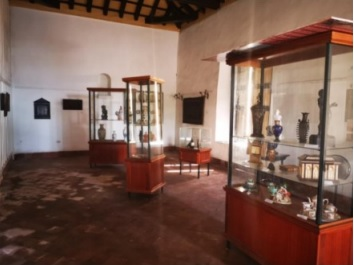
\includegraphics[width=8cm, height=6cm]{imagenes/sala_1.jpg}
        \caption{Sala 1}
        \label{imag:sala_1}
    \end{figure}

    En la sala 2 solamente se encuentran pinturas pertenecientes a la colección, estas poseen también condiciones de deterioro notables por el efecto de la humedad y del nivel de luz dentro del local.

    [Imagen de la sala 2]\newline
    Dentro de la sala 3 se localizan también varios objetos ubicados en pedestales mostrando colecciones de medallas y objetos personales del mismo Prat Puig y, además, vitrinas donde se hallan, principalmente, objetos de cerámica como platos, jarrones y cántaros.\newline
    [Imagen sala 3]\newline

    En el gráfico que se muestra a continuación se relaciona el valor cuantitativo de las principales formas en las que se exponen las piezas dentro de estas salas pertenecientes a la colección.

    \begin{figure}[H]
        \centering
        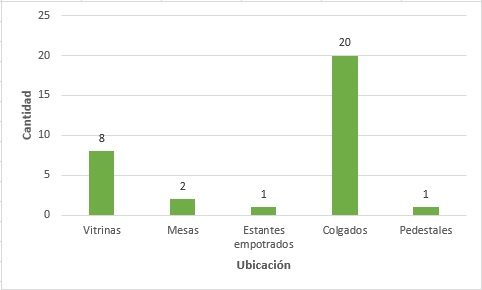
\includegraphics[width=10cm, height=6cm]{imagenes/formas expositivas.jpg}
        \caption{Ubicación piezas}
        \subcaption*{Fuente: Elaboración propia}
        \label{imag:ubicacion_piezas}
    \end{figure}

    Según la figura \ref{imag:ubicacion_piezas}, varios objetos están dispuestos dentro de vitrinas donde, al encontrarse protegido por paredes de cristal, se genera un microclima\footnote{microclima: según el diccionario Oxford, es el conjunto de las condiciones climáticas particulares de un lugar determinado, resultado de una modificación más o menos acusada y puntual del clima de la zona en que se encuentra influido por diferentes factores ecológicos y medioambientales.}, por lo que la condición ambiental en estas es diferente a la condición ambiental de la sala, de ahí la necesidad de incorporar nodos de tal manera que se tomen los datos dentro de estas vitrinas y, además, un nodo para la sala en general.

    \section{Arquitectura IoT y sus principales capas}\label{sec:arquitecturas}

    No existe una única definición universalmente adoptada, estándar, de Arquitectura de IoT; diferentes propuestas han surgido durante su desarrollo. Se abarcan tecnologías de comunicación, dispositivos de cómputo, sensores y actuadores \cite{ioT_en_Cosas_de_salud}.
    
    La arquitectura de IoT es principalmente desarrollada por capas, dígase, la arquitectura de 3 capas, la arquitectura de 5 capas, la arquitectura de Nube, la arquitectura de niebla y la arquitectura de computación de Borde, solo por mencionar algunas \cite{arquitecturaIEEE}.\\

    \begin{figure}[H]
        \centering
        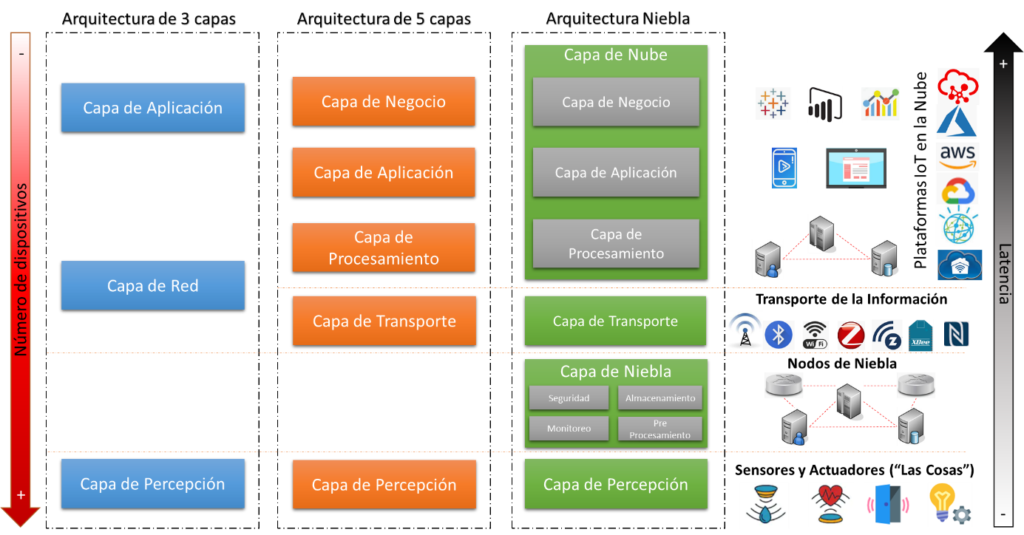
\includegraphics[width=8cm, height=5cm]{imagenes/Comparacion-arquitecturas-1024x535}
        \caption{Comparación arquitecturas}
            \subcaption*{Fuente: \cite{arquitecturaPaginaLuisGarcia}}
        \label{imag:comparacionArquitecturas}
    \end{figure}

    En la figura \ref{imag:comparacionArquitecturas} se desarrolla una comparación entre las arquitecturas de 3 capas, 5 capas y la arquitectura niebla.

    Según Ciberseguridad \cite{capasIoTciberseguridad}, la mayoría de estas arquitecturas de IoT se basan en fundamentos básicos:
    \begin{itemize}
        \item Dispositivos más inteligentes en una forma diferente.
        \item Red y puerta de enlace que permite que los dispositivos formen parte del IoT.
        \item Middleware que incluye espacios de almacenamiento de datos y avances en las capacidades de predicción.
        \item Aplicaciones de usuario final.
    \end{itemize}

    Existen varias arquitecturas, marcos de referencia o modelos conceptuales para IoT propuestos por organizaciones, comunidad académica y el sector empresarial. Las propuestas de arquitecturas pueden variar de autor en autor, en dependencia de la estructura del sistema IoT propuesto. Dichas arquitecturas son desarrolladas por capas en las que se agrupan los objetos, dispositivos, sensores, actuadores, entre otros. \cite{internetOfThingsStateOfTheArt} \cite{capasIoTciberseguridad}.\\

    En la figura \ref{imag:modelos_arquitecturas_iot} se representa una comparativa de algunos modelos basados en capas. Para propiciar una mejor comprensión de la figura \ref{imag:modelos_arquitecturas_iot} se desarrolló la tabla \ref{tab: referencias_capas} donde se muestra la relación de los autores referidos a las capas del IoT.

    \begin{table}[H]
        \centering
        \caption{Referencias figura \ref{imag:modelos_arquitecturas_iot}}
        \subcaption*{Fuente: Elaboración propia}
        \begin{tabular}{|l|l|}
        \hline
        \textbf{No. de Capas}    & \textbf{Referencias}                                                                                                                                              \\ \hline
        \multirow{2}{*}{3 capas} & \multirow{2}{*}{\begin{tabular}[c]{@{}l@{}}\cite{ref10} \cite{ref13} \cite{ref15}\\ \cite{ref16} \cite{ref19} \cite{ref25}\end{tabular}} \\
                                 &                                                                                                                                                                   \\ \hline
        4 capas                  & \begin{tabular}[c]{@{}l@{}}\cite{ref10} \cite{ref12} \cite{ref13}\\ \cite{ref19} \cite{ref16}\end{tabular}                          \\ \hline
        5 capas                  & \begin{tabular}[c]{@{}l@{}}\cite{ref9} \cite{ref10} \cite{ref13}\\ \cite{ref19} \cite{ref16}\end{tabular}                          \\ \hline
        Basado en SOA            & \begin{tabular}[c]{@{}l@{}}\cite{ref4} \cite{ref8} \cite{ref9}\\ \cite{ref15}\end{tabular}                                                        \\ \hline
        Basado en Middleware     & \cite{ref9}                                                                                                                                                \\ \hline
        6 capas                  & \cite{ref19}                                                                                                                                                        \\ \hline
        \end{tabular}
        \label{tab: referencias_capas}
    \end{table}

    \begin{figure}[H]
        \centering
        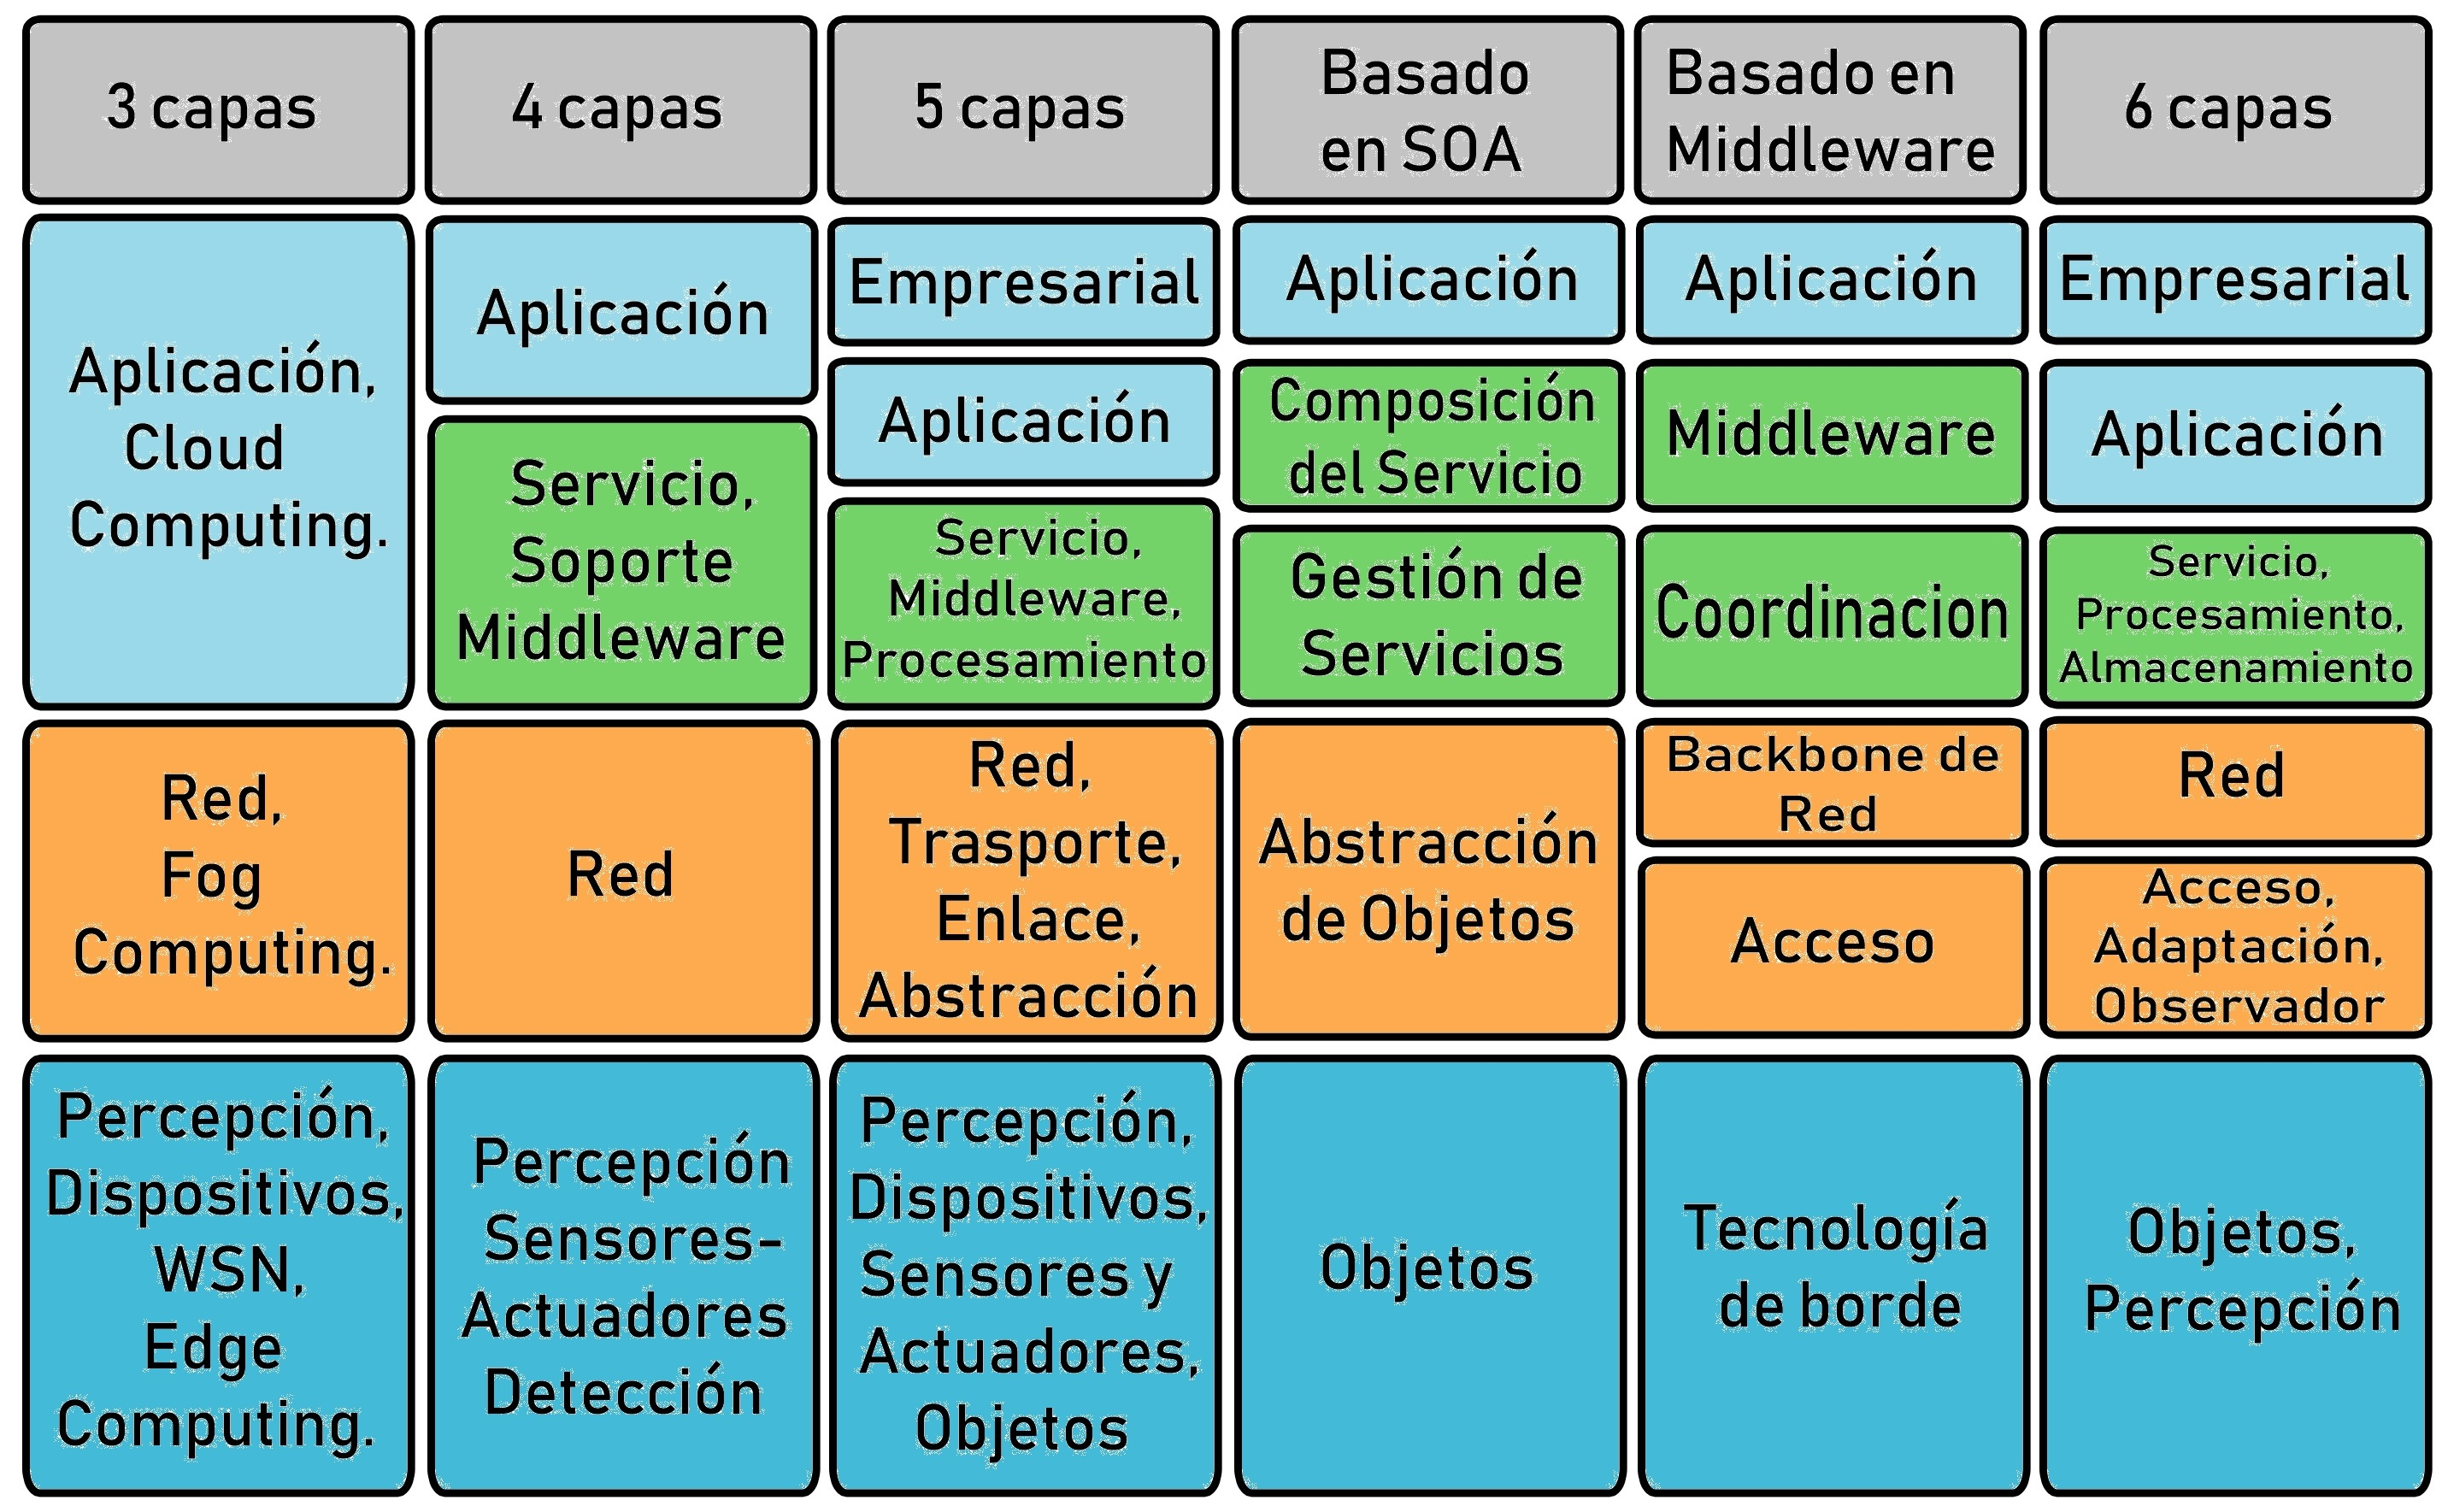
\includegraphics[width=15.6cm, height=9cm]{imagenes/capas.jpg}
        \caption{Modelos de arquitecturas IoT basados en capas}
        \subcaption*{Fuente: Elaboración propia}
        \label{imag:modelos_arquitecturas_iot}
    \end{figure}

    Desde el punto de vista de Ciberseguridad \cite{capasIoTciberseguridad} existen capas fundamentales dentro de la esctructura de IoT. En la tabla \ref{tab: capas_IoT} se detallan estas capas:

    \begin{table}[h]
        \centering
        \caption{Capas de IoT}
        \subcaption*{Fuente: \cite{capasIoTciberseguridad}}
        \begin{tabular}{|l|l|}
        \hline
        \rowcolor[HTML]{9698ED} 
        \textbf{Capas}                                                             & \textbf{Descripción}                                                                                                                                                         \\ \hline
                                                                                   &                                                                                                                                                                              \\
        \multirow{-2}{*}{Capa de percepción}                                       & \multirow{-2}{*}{Administra dispositivos inteligentes en todo el sistema.}                                                                                                   \\ \hline
        \begin{tabular}[c]{@{}l@{}}Capa de conectividad/\\ transporte\end{tabular} & \begin{tabular}[c]{@{}l@{}}Permite transferir datos desde la nube a los dispositivos\\ y viceversa, diferentes aspectos de las puertas de enlace\\ y las redes.\end{tabular} \\ \hline
        Capa de procesamiento                                                      & \begin{tabular}[c]{@{}l@{}}Controla y administra los niveles de IoT para optimizar\\ los datos en todo el sistema.\end{tabular}                                              \\ \hline
        Capa de aplicación                                                         & \begin{tabular}[c]{@{}l@{}}Ayuda en los procedimientos de análisis, control de\\ dispositivos e informes a los usuarios finales.\end{tabular}                                \\ \hline
        Capa empresarial                                                           & \begin{tabular}[c]{@{}l@{}}Deriva información y análisis de toma de decisiones\\ a partir de datos.\end{tabular}                                                             \\ \hline
        Capa de seguridad                                                          & \begin{tabular}[c]{@{}l@{}}Cubre todos los aspectos de protección de toda la\\ arquitectura de IoT.\end{tabular}                                                             \\ \hline
        Capa de borde                                                              & \begin{tabular}[c]{@{}l@{}}Funciona en un bode o cerca de la recopilación\\ de información del dispositivo.\end{tabular}                                                     \\ \hline
        \end{tabular}
        \label{tab: capas_IoT}
        \end{table}

    No obstante, según B. Mazon y A. Pan Olivo \cite{internetOfThingsStateOfTheArt}, dentro de las capas más importantes del IoT podemos encontrar:

    \begin{itemize}
        \item \textit{La capa de percepción} (Objetos/ Dispositivos/ SensorActuador/ WSN/ Edge Computing/ Sensado), digitaliza y transfiere datos a la capa de red, a través de canales seguros. Se localizan los objetos físicos, dispositivos sensores y actuadores utilizados para recopilar información del contexto. \cite{ref9}.
        \item \textit{La capa de acceso} (Adaptación/ Observador), comprueba la información que recibe de la capa de percepción, si está protegida o no contra intrusos y virus. Si hay algún ataque, no pasa los datos a la siguiente capa. También verifica la identidad y autenticación de los objetos. \cite{ref9} \cite{ref10}.
        \item \textit{La capa de Red} (Abstracción de Objetos/ Transporte/ Fog computing), transporta y transmite los datos, recopilados de la capa de percepción, hacia la cloud. Se localizan componentes de red (switch, router, Gateway, etc.), medios de comunicación y protocolos. También es responsable de aspectos de seguridad y el control de ataques. \cite{ref9} \cite{ref10}.
        \item \textit{La Capa Aplicación / Cloud Computing (CC)} en modelos de más de tres capas, puede dividirse en:
            \begin{itemize}
                \item \textit{Capa de procesamiento y almacenamiento, Soporte, o Middleware}. Permite a los programadores de aplicaciones IoT trabajar con objetos heterogéneos sin tener en cuenta una plataforma de hardware específica. Se encarga de integrar, almacenar, procesar y analizar datos, tomar decisiones y ofrecer servicios de protocolos de conexión de red. \cite{ref9}.
                \item \textit{La capa de aplicación}, define los servicios y funciones que proporciona la aplicación IoT implementada (hogar inteligente, ciudad inteligente, salud inteligente, etc.) a los clientes. Los servicios pueden variar para cada aplicación y depende de la información que se recopilan de los sensores. También se consideran aspectos de seguridad. \cite{ref9} \cite{ref10}.
                \item \textit{La capa empresarial}, tiene la responsabilidad de administrar y controlar el comportamiento de las aplicaciones, modelos de negocios y ganancias de IoT. También tiene la capacidad de determinar cómo se puede crear, almacenar y cambiar la información. Administra la privacidad del usuario y evita vulnerabilidades. \cite{ref9} \cite{ref10}.
            \end{itemize}
    \end{itemize} 

    \subsection{Propuesta de la Arquitectura IoT del Sistema}

    En base de los esquemas de arquitecturas propuestas, definimos el uso de la arquitectura del proyecto la cual se cimienta en la estructura de cuatro capas, considerando las diferentes capas que la componen:
    
    \begin{itemize}
        \item \textbf{Capa de Percepción: }Contiene todos los Nodos que se ubicarán en cada vitrina de la colección con sus sensores interconectados según sea la necesidad de cada vitrina y permitirán obtener los valores de las variables ambientales.
        \item \textbf{Capa de Transporte: }En esta capa se presenta el tipo de tecnología que se requiere utilizar para la transmisión de los datos recopilados por los sensores de los nodos con el concentrador principal que se encuentra en la Capa de Procesamiento, la comunicación entre ellos se realizá por Wifi y como protocolo de comunicación se pretende utilizar MQTT para mantener los valores actualizados constantemente.
        \item \textbf{Capa de Procesamiento: }Aquí se encuentra el concentrador principal con un servidor MQTT instalado,y con la Capa de Transporte se comunica con cada Nodo con sus sensores y contiene una base de datos local para almacenar todos los datos recopilados. Este concentrador a su vez envía estos datos de manera automática utilizando la conexión de Internet que se encuentra en el museo a una plataforma web de patrimonio universitario que se encuentra disponible en los servidores de la Universidad de Oriente y fue implementada por los autores Morejón y cols.\cite{morejon} utilizando una API en proceso de desarrollo. De igual forma en esta capa se podrán aplicar algoritmos de multicriterio que permitan analizar los datos y brindarles a los especialistas diferentes acciones.
        \item \textbf{Capa de Visualización: }En esta capa se encuentra la representación de todos los datos recopilados en la plataforma universitaria a los directivos o especialistas de la colección por navegadores web, sin embargo aunque esta es una alternativa de obtener esos datos, la principal novedad de esta investigación es la integración del IoT con la RA por lo que los especialistas que se encuentren dentro del museo podrán acceder a la información utilizando una aplicación móvil que se propone y utiliza la tecnología de RA para mostrar alertas y la información ambiental para cada vitrina o bien patrimonial, de igual forma desde la aplicación se podrá interactuar con la ficha técnica de cada elemento patrimonial para enviarlo a conservación o restauración. 
    \end{itemize}

    El alcance de este trabajo va dirigido a la explicación detallada de la Capa de Percepción, enfocándose en las características del microcontrolador y sensores a emplear según la necesidad, así como la Capa de Transporte donde se hace un análisis de los métodos y protocolos de comunicación empleados en el sistema.

    \subsection{Capa de Percepción}\label{subsec:capa_percepcion}

    Las SN (Sensor Network: Rede de Sensores) incluyen múltiples dispositivos (motes o nodos) equipados con transductores, actuadores y sensores que interactúan según la aplicación IoT \cite{hernandez}.
    Una SN puede estar formada por cientos o miles de nodos que se comunican entre sí y transmiten datos a otros dispositivos como el Gateway y a través de este se envían a un sistema distribuido o centralizado
    para su almacenamiento y procesamiento \cite{hernandez} \cite{lee}.

    Los sensores convierten estímulos físicos en señales eléctricas analógicas o digitales y según la señal se clasifican en acústicos, eléctricos, magnéticos, ópticos, térmicos y mecánicos \cite{hernandez}.
    También, se encargan de monitorear las características físicas, químicas o ambientales como: temperatura, humedad, movimiento, velocidad del viento, dirección del viento, nivel de Ph, electro conductividad, nivel de luz, entre otras \cite{lee}.

    La sucesión de sensores, en conjunto con el microcontrolador conforman la capa de percepción (figura \ref{imag:capa_percepcion}). 

    \begin{figure}[H]
        \centering
        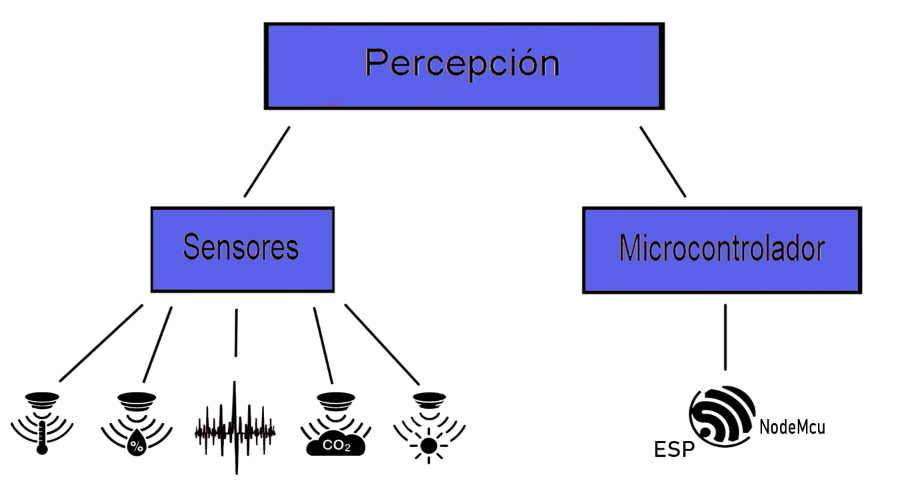
\includegraphics[width=8.5cm, height=4.5cm]{imagenes/perception_image.jpg}
        \caption{Diagrama funcional de captura de datos}
        \subcaption*{Fuente: Elaboración propia}
        \label{imag:capa_percepcion}
    \end{figure}

    \addcontentsline{toc}{subsection}{\hspace{1.3cm}1.4.2.1\hspace{5mm}Nodos}
    \textbf{1.4.2.1\hspace{5mm}Nodos}

    Los nodos que recopilarán los datos de cada vitrina estarán compuestos por el microcontrolador y los sensores encargados de tomar los valores medioambientales presentes teniendo en cuenta el material de las piezas expuestas dentro de cada una de las vitrinas.
    
    Estos nodos estarán ubicados también en las salas en aras de tomar datos de la habitación y relacionarlos con los obtenidos de las vitrinas.

    En base a esto, la tabla \ref{tab:correlacion_nodos} relaciona la variable a medir según la ubicación del nodo.

    \begin{table}[h]
        \centering
        \caption{Correlación de los nodos}
        \subcaption*{Fuente: Elaboración propia}
        \begin{tabular}{|l|c|l|c|}
        \hline
        \rowcolor[HTML]{9698ED} 
        \multicolumn{1}{|r|}{\cellcolor[HTML]{9698ED}Nodo} & \multicolumn{1}{r|}{\cellcolor[HTML]{9698ED}Ubicación}                      & Material objetos                                                                            & \multicolumn{1}{l|}{\cellcolor[HTML]{9698ED}Variable a medir}                                                                    \\ \hline
        1                                                  & \begin{tabular}[c]{@{}c@{}}General\\ Sala 1\end{tabular}                    & porcelana, barro, marfil                                                                    & \begin{tabular}[c]{@{}c@{}}temperatura, humedad,\\ polución, luminosidad,\\ CO2, vibraciones, salitre,\\ xilófagos\end{tabular}  \\ \hline
        2                                                  &                                                                             & bronce, barro, arcilla, piedra                                                              &                                                                                                                                  \\ \cline{1-1} \cline{3-3}
        3                                                  &                                                                             & colección numismática                                                                       &                                                                                                                                  \\ \cline{1-1} \cline{3-3}
        4                                                  &                                                                             & cerámica, madera, barro, bronce                                                             &                                                                                                                                  \\ \cline{1-1} \cline{3-3}
        5                                                  &                                                                             & \begin{tabular}[c]{@{}l@{}}madera, bronce, plata, cerámica,\\ porcelana, cuero\end{tabular} &                                                                                                                                  \\ \cline{1-1} \cline{3-3}
        6                                                  &                                                                             & barro, cerámica, plata                                                                      &                                                                                                                                  \\ \cline{1-1} \cline{3-3}
        7                                                  &                                                                             & bronce, marfil, madera                                                                      &                                                                                                                                  \\ \cline{1-1} \cline{3-3}
        8                                                  & \multirow{-7}{*}{\begin{tabular}[c]{@{}c@{}}Vitrinas\\ Sala 1\end{tabular}} & porcelana, barro policromado                                                                & \multirow{-7}{*}{\begin{tabular}[c]{@{}c@{}}temperatura, humedad,\\ luminosidad, vibraciones.\end{tabular}}                      \\ \hline
        9                                                  & \begin{tabular}[c]{@{}c@{}}General\\ Sala 2\end{tabular}                    & tela, madera                                                                                & \begin{tabular}[c]{@{}c@{}}temperatura, humedad,\\ polución, luminosidad,\\ CO2, salitre, xilófagos.\end{tabular}                \\ \hline
        10                                                 & \begin{tabular}[c]{@{}c@{}}General\\ Sala 3\end{tabular}                    & metal, plástico, tela, cuero, madera                                                        & \begin{tabular}[c]{@{}c@{}}temperatura, humedad,\\ polución, luminosidad,\\ CO2, vibraciones, salitre,\\ xilófagos.\end{tabular} \\ \hline
        11                                                 &                                                                             &                                                                                             &                                                                                                                                  \\ \cline{1-1}
        12                                                 &                                                                             &                                                                                             &                                                                                                                                  \\ \cline{1-1}
        13                                                 &                                                                             &                                                                                             &                                                                                                                                  \\ \cline{1-1}
        14                                                 & \multirow{-4}{*}{\begin{tabular}[c]{@{}c@{}}Vitrinas\\ Sala 3\end{tabular}} & \multirow{-4}{*}{cerámica (barro), piedra}                                                          & \multirow{-4}{*}{\begin{tabular}[c]{@{}c@{}}temperatura, humedad,\\ luminosidad, vibraciones.\end{tabular}}                      \\ \hline
        \end{tabular}
        \label{tab:correlacion_nodos}
    \end{table}

    Las variables ambientales a medir van estrechamente relacionadas con los sensores; estos sensores también fueron elegidos principalmente por su alto rango de mediciones ya que permiten diversos valores mínimos 
    y máximos permitiendo a su vez detectar cualquier inconveniente que pueda ser corregido mediante software sin necesidad de realizar calibraciones constantes en los laboratorios y se mantenga el sistema en invariable funcionamiento. 

    En el caso del microcontrolador lo que propone Alsuhly y cols.\cite{alsuhly} es utilizar como nodo un ESP32, un microcontrolador basado en el chip ESP8266 con bastante potencia para poder procesar la información de cada sensor de manera rápida,
    la conexion de este puede ser vía inalámbrica o por bluetooth al concentrador principal. En este caso se usará un NodeMCU, el cual es similar al ESP32 pero no contiene la interfaz bluetooth, esto permite abaratar más los costos de instalación ya que se necesitarán varios para cada vitrina de la colección.

    \subsection{Capa de transporte}\label{subsec:capa_transporte}

    Esta es la capa responsable del traslado de la data a través de los demás componentes del sistema estableciendo la comunicación necesaria desde la toma de valores ambientales hasta su análisis y muestreo.    
    Según \cite{internetOfThingsStateOfTheArt}, la capa de transporte es la que se encarga de transportar y transmitir los datos, recopilados de la capa de percepción, hacia la cloud. Se localizan componentes de red (switch, router, Gateway, etc.), medios de comunicación y protocolos. También es responsable de aspectos de seguridad y el control de ataques.
    
    Los datos se promueven a través de protocolos MQTT, HTTP y TCP/IP.
    
    \addcontentsline{toc}{subsection}{\hspace{1.3cm}1.4.3.1\hspace{5mm}Protocolo MQTT}
        \textbf{1.4.3.1\hspace{5mm}Protocolo MQTT}

    MQTT son las siglas MQ Telemetry Transport, aunque en primer lugar fue conocido como Message Queing Telemetry Transport. Es un protocolo de comunicación M2M (machine-to-machine) de tipo message queue. Está basado en la pila TCP/IP como base para la comunicación. En el caso de MQTT cada conexión se mantiene abierta y se “reutiliza” en cada comunicación. Es una diferencia, por ejemplo, a una petición HTTP 1.0 donde cada transmisión se realiza a través de conexión.
    MQTT fue creado por el Dr. Andy Stanford-Clark de IBM y Arlen Nipper de Arcom (ahora Eurotech) en 1999 como un mecanismo para conectar dispositivos empleados en la industria petrolera.
    Aunque inicialmente era un formato propietario, en 2010 fue liberado y pasó a ser un estándar en 2014 según la OASIS (Organization for the Advancement of Structured Information Standards). \cite{mqtt}\\

    \addcontentsline{toc}{subsection}{\hspace{1.3cm}1.4.3.2\hspace{5mm}Protocolo HTTP}
        \textbf{1.4.3.2\hspace{5mm}Protocolo HTTP}

    HTTP de sus siglas en inglés: “Hypertext Transfer Protocol”, es el nombre de un protocolo el cual nos permite realizar una petición de datos y recursos, como pueden ser documentos HTML. Es la base de cualquier intercambio de datos en la Web, y un protocolo de estructura cliente-servidor, esto quiere decir que una petición de datos es iniciada por el elemento que recibirá los datos (el cliente), normalmente un navegador Web. Así, una página Web completa resulta de la unión de distintos sub-documentos recibidos, por ejemplo: un documento que especifique el estilo de maquetación de la página Web (CSS), el texto, las imágenes, videos, scrips, etcétera.\\


    \addcontentsline{toc}{subsection}{\hspace{1.3cm}1.4.3.3\hspace{5mm}Protocolo TCP/IP}
        \textbf{1.4.3.3\hspace{5mm}Protocolo TCP/IP}

    La definición de TCP/IP es la identificación del grupo de protocolos de red que hacen posible la transferencia de datos en redes, entre equipos informáticos e internet. Las siglas TCP/IP hacen referencia a este grupo de protocolos:

    \begin{itemize}
        \item TCP: Es el Protocolo de Control de Trasmisión que permite establecer una conexión y el intercambio de datos entre dos anfitriones. Este protocolo proporciona un transporte fiable de datos.
        \item IP o protocolo de internet, utiliza direcciones series de cuatro octetos con formato de punto decimal (por ejemplo 75.4.160.25). Este protocolo lleva los datos a otras máquinas de la red.
    \end{itemize}

    El modelo TCP/IP permite un intercambio de datos fiable dentro de una red, definiendo los pasos a seguir desde que se envían los datos (en paquetes) hasta que son recibidos. Para lograrlo utiliza un sistema de capas con jerarquías (se construye una capa a continuación de la anterior) que se comunican únicamente con su capa superior (a la que envía resultados) y su capa inferior (a la que solicita servicios) \cite{tcp/ip}.

    %Así, esta arquitectura pretende servir de referencia para la implementación de servicios basados en IoT en el área de conservación de las piezas en los museos o instituciones con vista al desarrollo de entornos inteligentes.\\

    %\section{Sistema de comunicación}\label{sec: sistemaComunicación}

    \section{Condiciones que favorecen el ataque de insectos xilófagos}

    En el caso del control de la aparición de los xilófagos, como daño de origen biótico, no se encontró ningún sensor para medir el posible ataque de xilófagos, por lo que para anunciar la presencia de este tipo de anomalía se analizarán los restantes sensores y por correlación de datos será posible tenerlo en cuenta también.
    
    Por esto se realiza el análisis de las condiciones óptimas para la aparición de los mismos influyendo en la intensidad o severidad del ataque de estos insectos. Entre estos se pueden mencionar humedad, temperatura, entre otros \cite{ripa2004termitas}. 
    
    \subsection{Humedad}

    El contenido de agua de la madera constituye uno de los factores más importantes que favorecen el ataque de las especies xilófagas. Maderas con un contenido de humedad sobre el 15\% favorece las infestaciones de coleópteros xilófagos, acortando significativamente sus ciclos de vida lo que aumenta sus poblaciones y la posibilidad de reinfestaciones \cite{ripa2004termitas}, esto relacionado a que la acumulación de humedad se acentúa en construcciones con escasa ventilación, la que se debe incrementar en espacios interiores.

    Según Araquistain y col. \cite{monitoringMoisture} y Rodríguez y col. \cite{rodriguezcodigo}, el porcentaje de humedad óptimo para que crezcan los xilófagos está entre el 25 y el 55\% mientras que \cite{woodPreservation} plantea que, el rango de humedad idónea puede estar entre el 35 y el 50\%. Tomando estos porcentajes de humedad idóneos para la aparición de los xilófagos, se establece como valor máximo de humedad un 15\%.

    \subsection{Temperatura}

    Valores de temperatura idóneos para la aparición de xilófagos...


    %\section{Sistema de control de población}\label{sec: sistemaPoblacion}
    %Sensores PIR\\

    \addcontentsline{toc}{section}{Conclusiones}
    \textbf{\Large Conclusiones}\newline